\section{Technical Considerations}

\subsection{Data Extraction}

In order to extract content from multiple web pages, a web crawler will need to be created using the Python programming language. The group plans on using Scrapy, a Python library which will handle the ``visiting'' of websites, when provided with a sufficient list of hosts. Scrapy crawls through each directory within the host (as defined by the site's \textsl{robots.txt} file). After visiting a URL, the content will be extracted and analysed using the information retrieval methods available in the Python Natural Language Toolkit (NLTK) library.

\begin{figure}
  \centering
  \begin{minipage}{7cm}
    \centering
    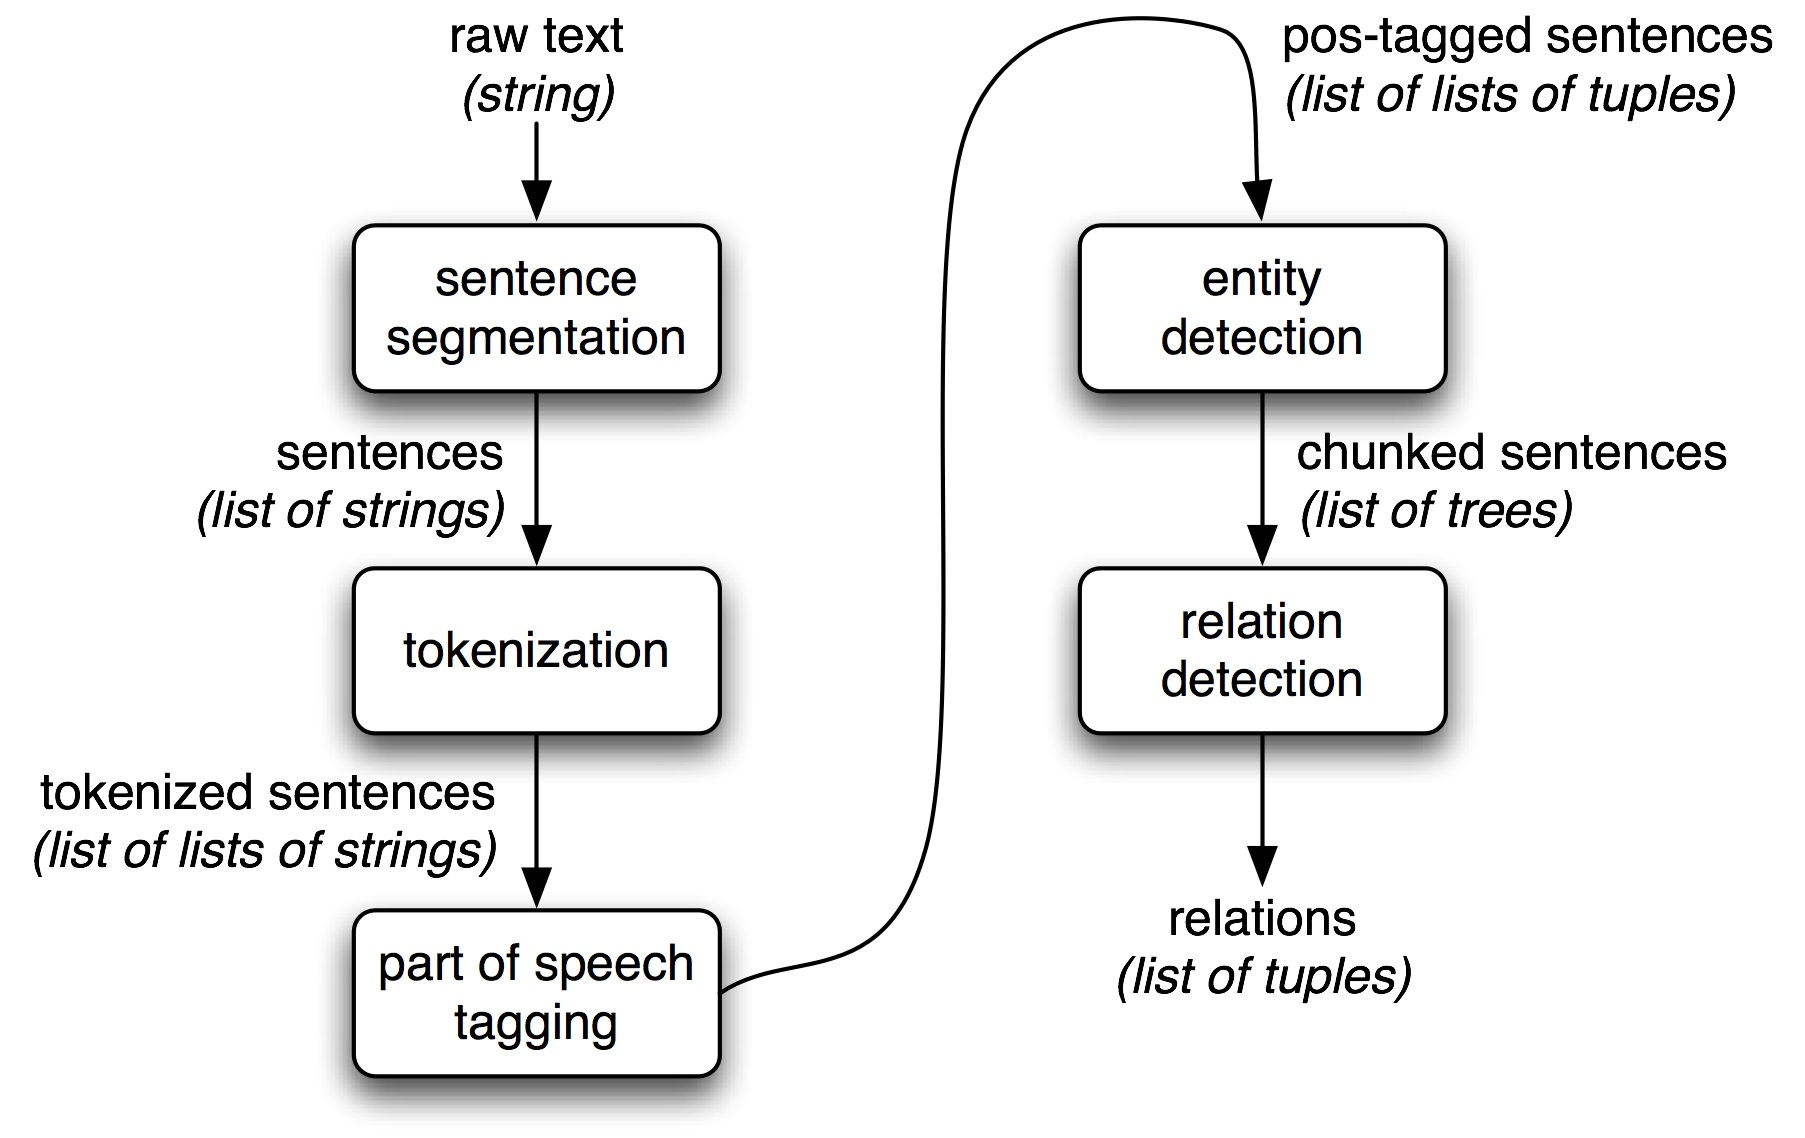
\includegraphics[width=7cm]{inc/ie-architecture.jpg}
    \caption{Python Natural Language Tookit Information Retrieval Flow Diagram}
    \label{fig:information_retrieval}
  \end{minipage}
\end{figure}

Many websites implement measures to prevent web crawlers from crawling due to the number of requests made as they utilise their server resources. Quite often, this results in the crawler being banned. However, the group can take the following measures to prevent this:

\begin{itemize}
  \item Disabling cookies may prevent getting banned, but only if it’s the method used by the website to detect crawlers
  \item Using Google cached pages instead of visiting the websites directly
  \item Using different IP addresses by rotating from a list when making a request to the same host
  \item Setting a delay between requests
\end{itemize}

%\clearpage

\subsection{Sentiment Analysis}

Once the user's online content has been extracted, it will then placed into one of the following categories: negative, positive or neutral. This can be achieved by performing sentiment analysis on the content. However, the app's back-end has to be first be trained by supplying sufficient training data.

The language used for the sentiment analysis will be Python. Moreover, the group will also make use of the Natural Language Toolkit (NLTK) Python library.

\subsubsection{Data Collection \& Pre-Processing}

The first step is to collect existing positive, negative and neutral content and store them in an array.

\begin{figure}[h!]
  \centering
  \begin{minipage}{14cm}
    \centering
    \inputminted[fontsize=\footnotesize]{python}{inc/snippets/collection.py}
    \caption{Content Collection}
    \label{fig:sentiment_analysis_step1a}
  \end{minipage}
\end{figure}

These words are then collected into a single list of tuples, each of which containing two elements.

\begin{figure}[h!]
  \centering
  \begin{minipage}{14cm}
    \centering
    \inputminted[fontsize=\footnotesize]{python}{inc/snippets/collection_iteration.py}
    \caption{Content Pre-Processing}
    \label{fig:sentiment_analysis_step1b}
  \end{minipage}
\end{figure}

\subsubsection{Classifier Creation}

Once sufficient content has been attained, a list of each word extracted from all the content needs to be collected and then ordered based on frequency of occurrence. This can be done by initially collecting all words and associating a frequency of occurrence to each and then ordering the list based on the frequency value. 

\begin{figure}[h!]
  \centering
  \begin{minipage}{14cm}
    \centering
    \inputminted[fontsize=\footnotesize]{python}{inc/snippets/classifier.py}
    \caption{Word Frequency}
    \label{fig:sentiment_analysis_step2a}
  \end{minipage}
\end{figure}

To create the classifier, relevant features needs to be captured via a feature extractor.

\begin{figure}[h!]
  \centering
  \begin{minipage}{14cm}
    \centering
    \inputminted[fontsize=\footnotesize]{python}{inc/snippets/classifierB.py}
    \caption{Feature Extraction}
    \label{fig:sentiment_analysis_step2b}
  \end{minipage}
\end{figure}

A training set will then be created using the NLTK library. Furthermore, a classifier object can be instantiated.

\begin{figure}[h!]
  \centering
  \begin{minipage}{14cm}
    \centering
    \inputminted[fontsize=\footnotesize]{python}{inc/snippets/classifierC.py}
    \caption{Classifier Training}
    \label{fig:sentiment_analysis_step2b}
  \end{minipage}
\end{figure}

\subsubsection{Classifier Testing}

Now that the classifier has been created and trained, the sentiment analyser can be tested.

\begin{figure}[h!]
  \centering
  \begin{minipage}{14cm}
    \centering
    \inputminted[fontsize=\footnotesize]{python}{inc/snippets/classify.py}
    \caption{Classifier Testing}
    \label{fig:sentiment_analysis_step3}
  \end{minipage}
\end{figure}

\clearpage

\subsection{Pattern Matching and Image Recognition Algorithms}

  This section contains information on the pattern matching and image recognition algorithms that could utilised in the solution in order to help individuals devise a strategy for which data linked with them could be used for.

  \subsubsection{Pattern Matching}

    The bitap algorithm is an approximate or exact string matching algorithm that is one of the underlying algorithms of the UNIX ``agrep'' utility~\cite{}. It determines whether a given text contains a substring which is equal to a given pattern, where approximate equality is defined in terms of the Levenshtein distance – a complementary algorithm which determines how many changes must be made to a string or phrase in order to turn it into another string or phrase~\cite{}. In comparison to other algorithms, bitap does most of the work with bitwise operations, thus making it run super-fast.
      %This algorithm's library is available at https://code.google.com/p/google-diff-match-patch/.

    \begin{figure}
      \centering
      \begin{minipage}{10cm}
        \centering
        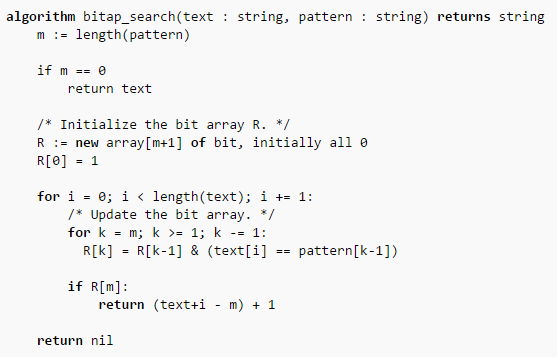
\includegraphics[width=10cm]{inc/bitap_algorithm.png}
        \caption{Bitap Algorithm Pseudocode}
        \label{fig:bitap_algorithm_pseudocode}
      \end{minipage}
    \end{figure}

  \subsubsection{Application}

    The solution will require access to two predefined datasets for classifying the information returned by search engine. The first dataset contains some sensitive keywords that will make a significant influence on public impression, such as drug abuse or achievement. The other dataset stores the words with a neutral, negative or positive emotion, and each word has a corresponding score, for example: disappointment with score -5, humiliation with score -8, honour with score +8 and success with score +6. 

      The steps for implementing this algorithm are as follows:
      \begin{enumerate}
        \item Search website articles for sensitive keywords and their relative location
        \item Search for ``emotional words'' that appear within the spatial locality of the sensitive keyword
        \item Calculate the score of the article or website based on the number of emotional words found
      \end{enumerate}

  \subsection{Image Recognition}

    \subsubsection{Description}

      Affine scale-invariant feature transform (or ASIFT) is computer vision algorithm that is used to detect and describe local features in images. It is regarded as an efficient method for determining matches between two arbitrarily-selected points within two widely separated views. Moreover, ASIFT is capable of finding a correspondence, even for pixels within an area with certain uniform properties, such as similar colours and textures~\cite{}.

      \begin{figure}
        \centering
        \begin{minipage}{12cm}
          \centering
          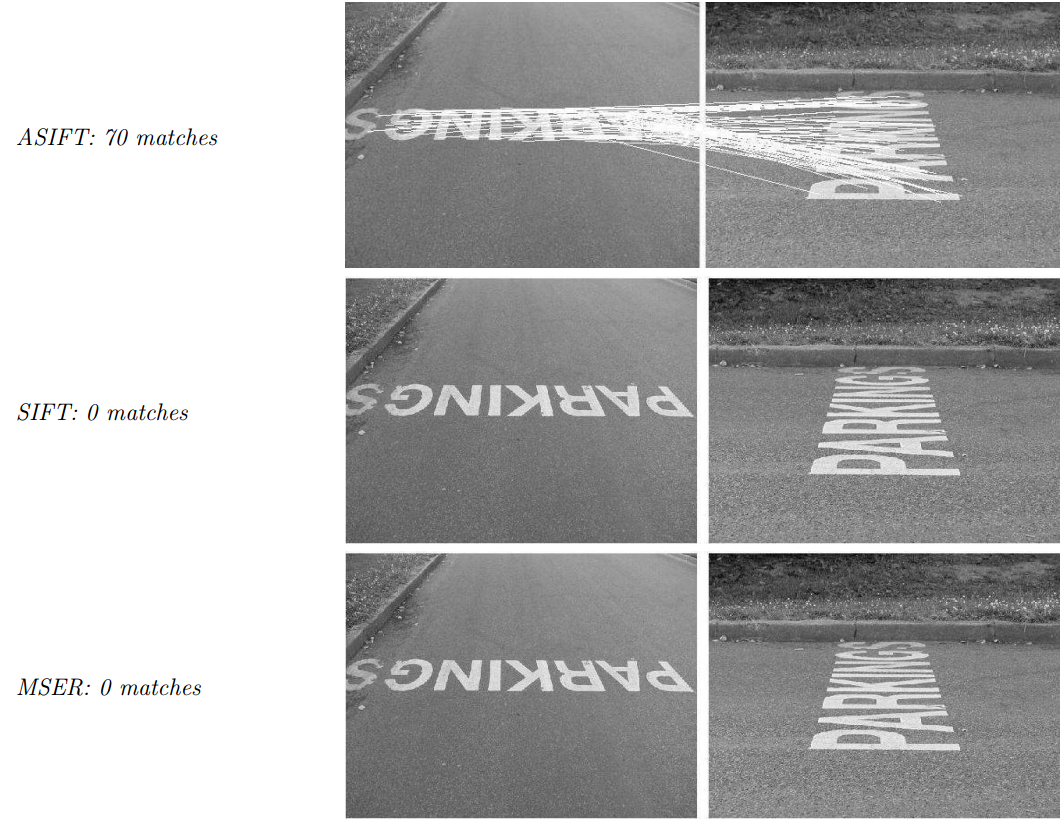
\includegraphics[width=12cm]{inc/image_recognition_comparison.png}
          \caption{Comparison of Image Recognition Algorithms}
          \label{fig:image_recognition_comparison}
        \end{minipage}
      \end{figure}

    \subsubsection{Application}

      During the text processing stage, a pattern matching algorithm can attempt to detect the purpose of an article or website. If it is determined that the page is an advertisement, then the image and face recognition algorithm can attempt to match the image with the relevant person's face. Once matched, a check can be carried out to determine whether or not the website has the right to use the portraiture.

\clearpage

\subsection{Encryption}

Data and device encryption are critical pieces of an overall mobile security initiative. Implementing encryption is vital to ensuring that sensitive data is kept safe. We will tackle mobile data encryption from two angles: data on devices and data transmitted to and from those devices.

\subsubsection{Data encryption techniques for on-device data}

The latest version of the Android OS offers several Android enterprise features, including on-device encryption (as long as users specifically enable it on their devices). And apps such as WhisperCore make it possible to fully encrypted on-device data on devices running older versions of Android.

When device encryption is enabled, the entire file system is protected, but turning encryption on doesn't mean other file systems are protected. Some Android devices have microSD cards, which have to be deliberately secured. MicroSD cards also make the media difficult to plug into other devices, because both devices need the same keys to use the media. Therefore, this App must be installed in the internal storage of a mobile device.

\subsubsection{ Data encryption techniques for transmitted data}

We should also make sure that any sensitive data transmitted between mobile devices and the enterprise is encrypted.

Mobile Device Management (MDM) is like adding an extra layer of security and ensuring a way to monitor device related activities. MDM provides device platform specific features like device encryption, platform specific policies, SD Card encryption. Geo-location tracking, connectivity profiles (VPN, Wi-Fi, Bluetooth) and plenty other features are part of MDM Suite.

Transport Layer Security (TLS) and its predecessor, Secure Sockets Layer (SSL), both of which are frequently referred to as ``SSL'', are cryptographic protocols designed to provide communications security over a computer network. Several versions of the protocols are in widespread use in applications such as web browsing, email, Internet faxing, instant messaging, and voice-over-IP (VoIP). Major websites (including Google, YouTube, Facebook and many others) use TLS to secure all communications between their servers and web browsers.

The primary goal of the TLS protocol is to provide privacy and data integrity between two communicating computer applications. When secured by TLS, connections between a client and a server will have one or more of the following properties:

The connection is private because symmetric cryptography is used to encrypt the data transmitted. The keys for this symmetric encryption are generated uniquely for each connection and are based on a secret negotiated at the start of the. The server and client negotiate the details of which encryption algorithm and cryptographic keys to use before the first byte of data is transmitted. The negotiation of a shared secret is both secure and reliable.

The identity of the communicating parties can be authenticated using public key cryptography. This authentication can be made optional, but is generally required for at least one of the parties.The connection is reliable because each message transmitted includes a message integrity check using a message authentication code to prevent undetected loss or alteration of the data during transmission.
